\section{Motivation and Research Overview}
\label{sec:motivation}

As our title suggests, \samir{best to refer to intro than title} there are  three key aspects to our vision: {\em
flexibility}, {\em wireless}, and the use of {\em free-space optics} in DC
networks.  We begin by arguing why  each of these aspects is needed before
 providing a high-level view of our proposed  architecture.


\subsection{Case for Flexibility in Datacenters} 
 %The critical role that datacenter performance plays has motivated several
 %efforts in the research literature. 
 Our focus in this paper is on the inter-rack fabric connecting different
top-of-rack (ToR) switches. At a high level, we can classify existing 
 designs along two axes:   (1) the extent of oversubscription 
  and (2)  flexibility (if any) to reconfigure links. 



\begin{wraptable}{r}{10cm}
\vspace{-0.5cm}
\begin{footnotesize}
\begin{tabular}{p{2cm}|p{2cm}|p{1.5cm}|p{3cm}}
Category &  Backbone  	&  Flexibility   & Notes \\ \hline
Leaf-Spine (e.g.,~\cite{}) 	& 	Wired, oversubscribed	& None 	 & Poor performance \\ \hline		
Full bisection bandwidth  (e.g.,~\cite{fattree,vl2})	& 	Wired, no oversubscription	& None 	 &  High cost +  cabling complexity, no incremental expandability \\ \hline		 
 %All optical  (e.g.,~\cite{OSA,proteus})	& 	All-Optical  	&  ?? 	 &  High cost, cabling \\ \hline		
Wireless augmentation   (e.g.,~\cite{60ghz,3db})	& 	Wired, oversubscribed 	& Few 60Ghz links 	 &  Low range, bandwidth \\ \hline		
Optical augmentation   (e.g.,~\cite{cthrough,OSA})	& 	Wired, oversubscribed 	& Single optical	 &  Limited flexibility, Single point of failure \\ \hline		
\ArchName vision 	& 	None  	& Steerable FSO  	 &  Not commodity yet  
\end{tabular}
\end{footnotesize}
\vspace{-0.3cm}
\caption{Taxonomy of datacenter network architectures and recent research proposals}
\label{tab:taxonomy}
\end{wraptable}

%% taxonomy of existing 
Table~\ref{}  summarizes prior work along these two key dimensions.
Traditional  static topologies such as leaf-spine fabrics~\cite{}  or fat-tree
architectures~\cite{} represent extremes in the space of  cost-performance
tradeoff.   Additionally, such  structured graphs impact  incremental
expansion~\cite{jellyfish}.  Recent measurements show that the DC traffic
patterns  exhibit hotspots of inter-rack activity with  a few ``heavy''
flows~\cite{flyways,cthrough,vl2}.  These motivated  
 designs where an oversubscribed core is {\em augmented} with a {\em few} 
 flexible  optical connections~\cite{} or wireless links~\cite{}.
 %% Why isnt existing augmentation good enough While we build on these
%data-driven insights that introduced the case for a flexible  DC design,  
  However, these are limited in the degree of flexibility and introduce
  additional challenges.
  Optical solutions create  a single point of failure,  
  and  cannot handle other one-to-many or
many-to-one demand patterns~\cite{flyways}. Wireless links,
 on the other hand,  are fundamentally 
limited in the capacity and range; e.g., even recent solutions cannot 
 provide more than \plsfill Mbps or \plsfill meters. Finally, they inherit 
   the cost and cabling complexity of the wired ``core'' they seek to extend. 

 
%Our vision takes the case for flexibility to its logical extreme. 
Rather than incrementally improve  an oversubscribed network, we posit that
flexibility, if designed suitably, can obviate the need for overprovisioning
and the need for a static backbone! This can provide a dramatically improved
point in the cost-performance tradeoff.  Furthermore, this flexibility can
enable energy savings by selectively shutting down links depending  on the
load~\cite{elastictree,googleisca}. 

\begin{wrapfigure}{r}{0.5\textwidth}
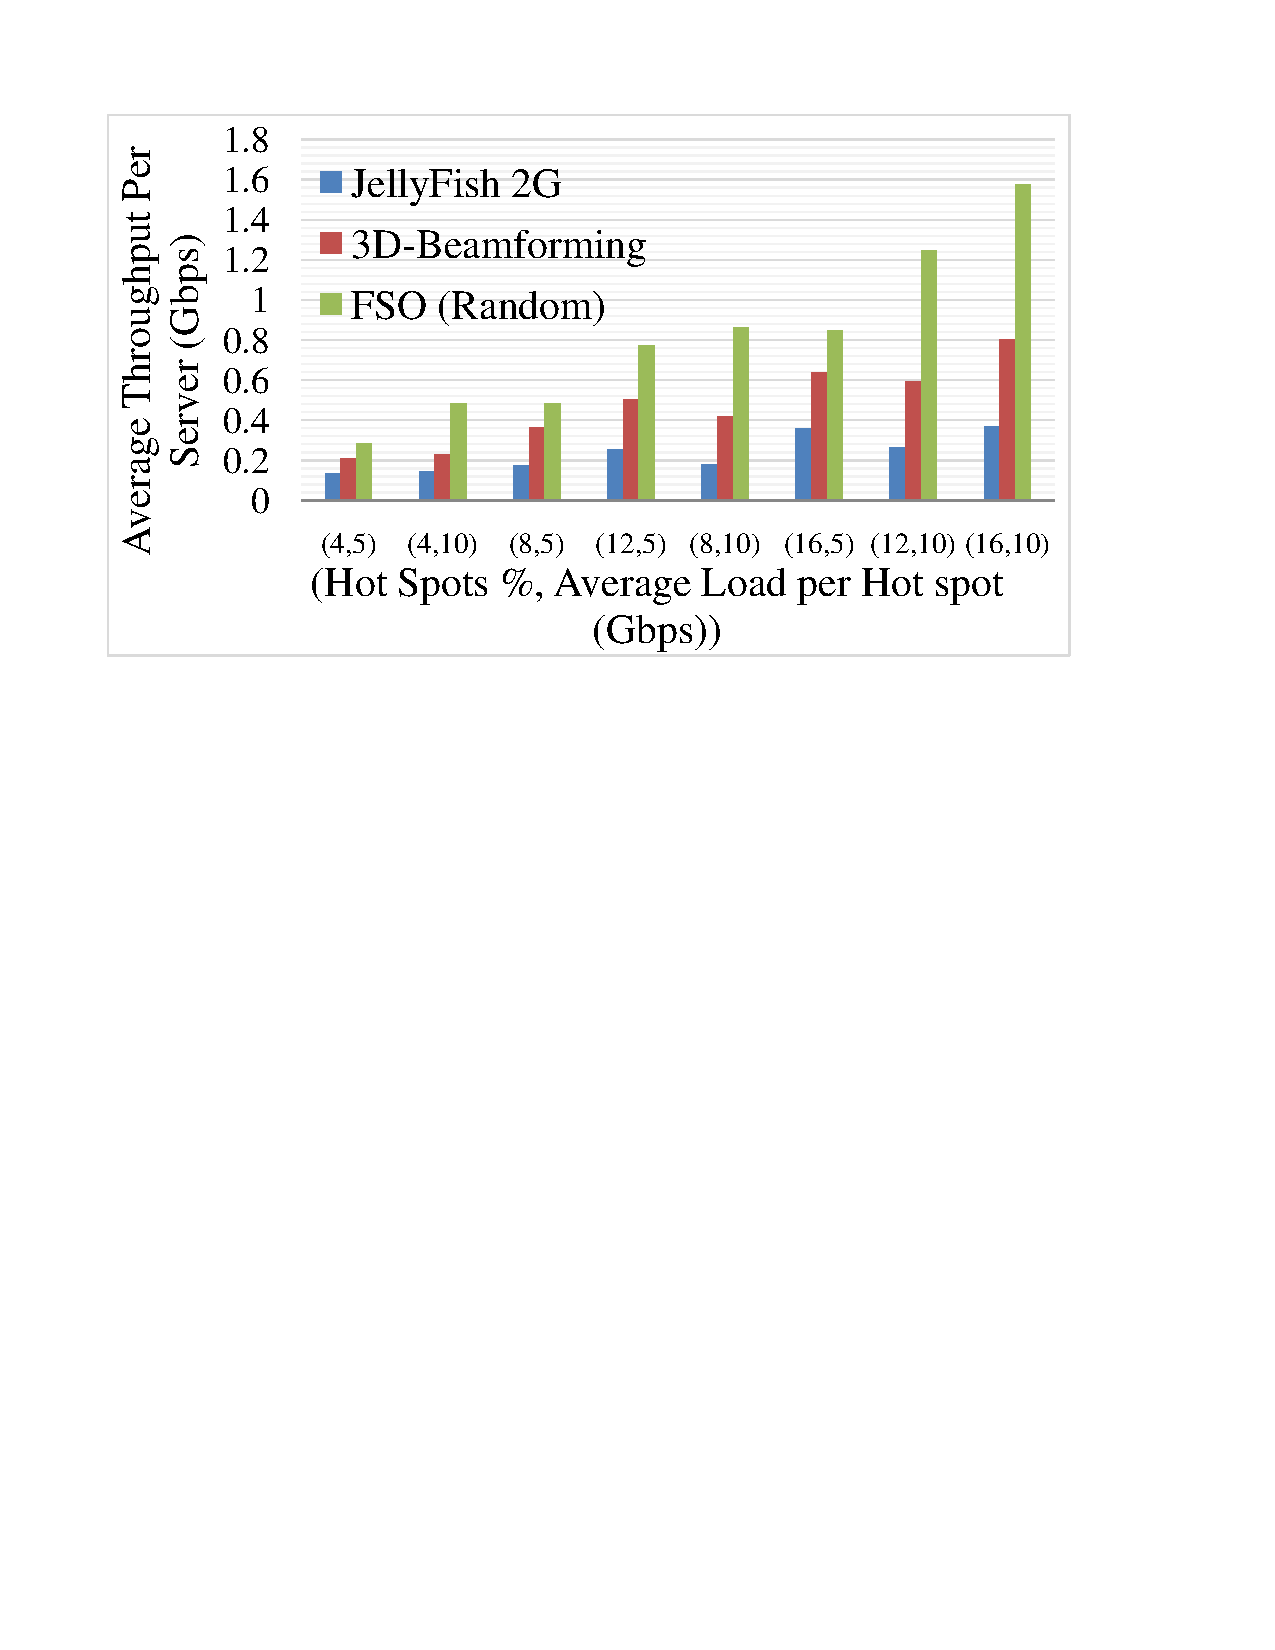
\includegraphics[width=220pt]{../hotnets13/Figures/Hotspots.pdf}
\caption{The case for flexibility -- it can provide performance comparable to a full bisection bandwidth 
 network with a lot less equipment and even get rid of aggregation layers. PLACEHOLDER from hotnets}
\label{fig:flexibility}
\end{wrapfigure}

%% Figure to show flexibility can get close to optimal
 To provide the basis for this intuition, we consider an abstract 
 model of a {\em flexible} datacenter as follows.  We consider a data center 
of 20 racks, where each rack has $\NumMachinesPerRack$ machines. We use 1Gbps $2\times \NumMachinesPerRack$-port
switches, as in FatTree architectures.  The ToR (top of rack) switches
 use $\NumMachinesPerRack$ ports for the machines, and the remaining $\NumMachinesPerRack$ ports for
inter-switch connections. The non-ToR switches use all their ports for
inter-switch connections. Our fixed architecure for (a) is based on a
random graph (of inter-switch connections) over $XX$ number of
switches, and delivers a performance of $ZZZ$ flow-completion time.
We generate $\DegreeFlex$-flexible architecture as follows: We allow $\DegreeFlex$ ports
of each ToR switch and $2\times\DegreeFlex$ ports of each non-ToR switch to be
``reconnected'' at each epoch; the interconnections between remaining
ports are random but {\em fixed}. Thus, higher the value of $\DegreeFlex$, more
flexible is the architecture. We also consider $\NumPortsPerToR$-ToRFlexible
architectures, wherein we use only ToR switches with $\NumPortsPerToR$ ports each;
 $\NumMachinesPerRack$ ports of these ToR switches are connected to the rack machines, 
and the remaining $\NumPortsPerToR-\NumMachinesPerRack$ ports are reconnected at every epoch.


%\vyas{not sure we want to show fattreee is underutilized since that requires real data?}
 Figure~\ref{fig:flexibility} shows that by increasing the degree of flexibily \plsfill.

\subsection{Case for Wireless via Free-Space Optical Communications}
 %talk about cabling,  power cooling  
\myparaq{Why wireless} To realize such a flexible fabric, conceptually we need
a reconfigurable ``patch-panel''  between  pairs of racks~\cite{sdnpatch}. Of
course, such a big-switch abstraction is infeasible: (1) it requires very high
fanout ($\NumRacks \times \DegreeFlex$, where $\NumRacks$ is the number of
racks and $\DegreeFlex$ is the number of flexible links at each ToR) and
backplane  switching capacity; and (2)
the  cabling complexity  would be prohibitive and create
operational overheads w.r.t failures, and cooling/airflow
considerations~\cite{}.  For similar reasons, traditional optical
 switching is also not viable.  Finally, this giant switch 
  introduces a single-point of failure~\cite{osa,proteus,helios}. 
 To avoid the need for such a massive switch, 
 we turn to  {\em reconfigurable wireless} links between the  ToR switches.\footnote{Note that we are not proposing a fully wireless data center~\cite{cornell}; our focus is on the ``inter-rack'
fabric.}

 % with  each ToR switch 
% equipped with $\DegreeFlex$ wireless transceivers as shown in
%Figure~\ref{fig:vision}.


%% wireless is not good enough hence fso
\myparaq{Why FSO} The seemingly natural  solution then is 
 traditional radio-frequency (RF) wireless technologies (e.g., 60GHz).
Unfortunately, these  have  many fundamental performance 
limitations: (1)  RF links produce a
large interference footprint due to a wide beamwidth, even with new ``ceiling
mirror'' architectures~\cite{3db}; \samir{This blames one paper only. This does
not argue why we are discounting every form of RF. Recall the comment from
hotnets reviewer. I can fix this. But the real argument is somewhat involved -- more than a oneliner.}  (2) The beam-steering  technologies
 to implement flexibility are  slow and
inaccurate~\cite{3db} and increase the interference
footprint~\cite{phased-arrays-rf}; \samir{Need to rephrase, overly sweeping.} 
and (3) The data rates of RF links fall off
rapidly with distance~\cite{3db} and the use 
 of  higher transmit power to increase the range 
 will increse interference and is limited by regulations~\cite{}.
To overcome these limitations, we leverage a somewhat non-standard wireless 
technology---free-space optics (FSO) that uses modulated visible or
infrared (IR) laser beams~\cite{kedar}.\footnote{Unlike traditional optical
links, the laser beam in FSO is not enclosed in a glass fiber, but transmitted
through the air (and hence  ``free space'').}  
%In contrast to RF,
%FSOs offer a lower interference footprint and much higher range and datarates.
 We elaborate on the advantages of FSO vs.\ RF in Section~\ref{sec:fso}.

\eat
{
There are two main benefits of FSO
compared to traditional RF technologies: 
% that make it a promising candidate for data centers:
%
\begin{packeditemize} \item {\em Low Noise and Interference.}  Unlike RF,
FSO links do not suffer from multipath fading or \blue{EM} noises~\cite{}.
Moreover, FSO beam divergence is  orders of magnitude narrower than RF
 (in the order of milliradians; 1 milliradian = $0.0573^\circ$). This
reduces `interference footprint' to a negligible level.  Thus, FSO
communications from multiple senders do not interfere, unless they are aligned
to the same receiver (which is easy to avoid).

 \item   {\em High Data Rates over Long Ranges:}  Optical links 
 provide significantly higher data rates than any  RF
technology as they use of  higher frequencies and are not restricticted by 
regulatory restrictions~\cite{kedar}. Coupled with  lower
attenuation, FSO links can offer Gbps--Tbps rates at long distances (several kms) even
with modest transmit power (few watts)~\cite{kedar,fsona,mustafa2013reintroducing}.

%%
%Commercially available FSO devices already offer data rates of
%2.5~Gbps~\cite{fsona}, and demonstration systems even report data
%rates in the order of Tbps~\cite{mustafa2013reintroducing} -- both for
%long distance (in the order of km) links.
\end{packeditemize}
}


\subsection{Architecture and Proposed Research}
 
\begin{wrapfigure}{r}{0.4\textwidth}
\label{fig:benefits}
\vspace{-0.4cm}
\centering
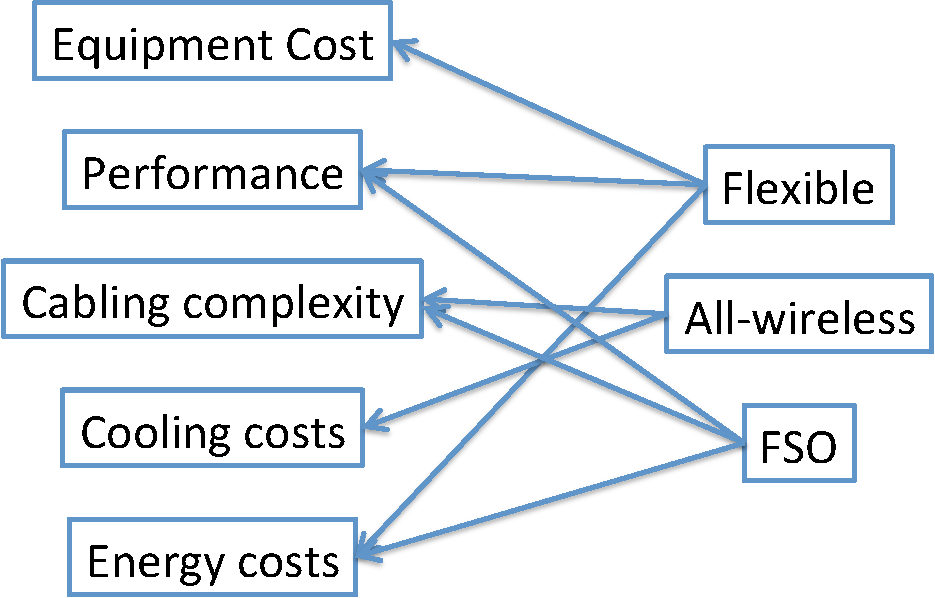
\includegraphics[width=150pt]{PPTFigs/benefitidea.pdf}
\caption{Overview of the key concepts underlying \ArchName and how they benefit different aspects 
 of datacenter considerations from Section~\ref{sec:intro}}
\label{fig:benefits}
\vspace{-0.4cm}
\end{wrapfigure}

%% revisit the architecture overview

%% benefits

Combining the above arguments leads us to the architecture   
in Figure~\ref{fig:vision}.  We eliminate the need for a wired backbone network
and rely on a reconfigurable FSO-based wireless fabric.  Each ToR switch is
equipped with a  pre-specified number of FSO devices and  each FSO device
assembly is capable of precise/fast steering to connect to  target
 ToRs. 
 % To establish an {\em obstruction-free} optical path, the space
 above the racks is a natural choice for laser propagation as this
 space is roughly free from obstruction~\cite{samirpic}.  The FSO
 transceivers will be anchored on the top of the rack and connected to
 the ToR switch.  \blue{To ensure that the devices themselves do not
   obstruct each other, we propose use of ceiling mirrors as
   in~\cite{3db} (and possibly additional mirrors on the beam path).}

 The DC management layer  intelligently
reconfigures these devices  to adapt to  changing network requirements.
 Figure~\ref{fig:benefits} summarizes  how the three key aspects of
\ArchName---flexibility, all-wireless, and use of FSOs--- benefit different
considerations of DC network design: (1) Flexibility  ensures high-performance
with lower cost  and  enables energy reduction~\cite{}; (2) A wireless  fabric
eliminates concerns about cabling complexity and  interference with
cooling~\cite{hpcabling}; and (3) Using FSOs eliminate performance concerns for
a wireless network that might arise from range and  interference constraints. 


% and also
%ensuring high performance and reliability in the presence of network flux;
%e.g., during reconfigurations or local link dynamics.


%% roadmap
 With this context,  we discuss the three broad research thrusts we need to
address to turn the benefits (Figure~\ref{fig:flexibility},\ref{fig:benefits})
into reality: (1) {\bf feasibility of FSOs for \ArchName
(Section~\ref{sec:fso})};  (2) {\bf foundations of flexible topology design
(Section~\ref{sec:topology})}; and (3) {\bf effective datacenter management
(Section~\ref{sec:system}).}

\hg{Need summary of cost-performance results from hotnets.}

\eat
{
\begin{packeditemize}
\item {\bf Feasibility of FSOs for \ArchName (Section~\ref{sec:fso}):}
 Because we envision a new use-case for FSOs, we need to establish the
feasibility of cost-effective (i.e.. commoditizable), small form-factor, 
and rapidly steerable FSO designs;  

\item {\bf Foundations of flexible topology design (Section~\ref{sec:topology}):}
  Ther are  practical constraints on the timescale-range tradeoffs of 
 steering mechanisms and  we need formal models to reason about  flexible
topology design subject to such steering and other cost constraints; and

\item {\bf Effective datacenter management (Section~\ref{sec:system}):}
 We need to address practical system design challenges in managing a fundamentally
dynamic network. 

\end{packeditemize}
}

% For each thrust, We discuss the challenges and our proposed research  in the rest of the proposal. 

\vyas{revisit these bullets to be consistent with intro of each section}

\eat
{
\vyas{need better phrasing here }

%\begin{packedenumerate}
%\item
\mypara{Feasibility of FSOs for \ArchName (Section~\ref{sec:fso})}
Traditional  use-cases for  FSOs  have a very different set of operating
constraints and requirements compared to DCs. For instance, they are mostly
designed to create static, outdoor links and are engineered to deal with
environmental  effects (e.g., scintillations)~\cite{}. Thus are bulky,
high-power,  and do not require rapid/precise reconfiguration.  In the DC
context, we need a small form factor (e.g., to pack more FSOs on each ToR) and
low power.  Consequently,  we need  (1) a small cost-effective, and
energy-efficient FSO device that can deliver 10-100Gbps data rate and (2)
mechanisms that will steer the laser beam with extreme precision (within
microradians) with low latency (order of few tens of milliseconds).

% We address the above challenges in {

\mypara{Foundations of flexible topology design (Section~\ref{sec:topology})} Due to the
limited steerability of the \blue{considered} steering mechanisms, we need to
{\em pre-configure} the steering mechanism of each FSO device (by pre-aligning
or pre-orienting it) to a set/range of other FSO devices. This
pre-configuration determines the set of fixed candidate links, from which the
active links are chosen in real-time (called {\em reconfiguration}) depending
on the prevailing traffic.
\vyas{need to rephrase this ..}

% We address the pre-configuration problem in {\bf
%  Section~\ref{sec:top}}, and the reconfiguration problem along with
%its related challenges in \bf{Section~\ref{sec:system}.}

\mypara{Effective datacenter management (Section~\ref{sec:system})} Finally, we
need to address practical system design challenges in the  management layer. To
this end, we leverage recent advances in software-defined networking  (SDN) for
fine-grained control over the network. However, we need to scalable
reconfiguration algorithms and mechanisms that guarantee performance and
consistency in the face of network/link dynamics.  Furthermore, an
all-wireless vision   means that we cannot rely on out-of-band control
channels, and thus we need new wireless control channels as well.  
}
 
%\end{packedenumerate}

